%!TeX shellEscape = restricted
%!TeX enableSynctex = true
\documentclass[11pt]{article}
\usepackage{url,amsmath,amsfonts}
\usepackage[capitalise,noabbrev]{cleveref} %
\crefname{equation}{}{} %
%\usepackage{minted} %If require code snippets, turn back on
\usepackage[nohead]{geometry}
\usepackage{tikz}
\usetikzlibrary{decorations.pathreplacing,angles,quotes,calligraphy}
\usepackage{graphicx}

%Some macros
\newcommand{\set}[1]{\ensuremath{\left\{{#1}\right\}}}
\newcommand{\R}{\ensuremath{\mathbb{R}}}
\newcommand{\D}[1][]{\ensuremath{\boldsymbol{\partial}_{#1}}}
\newcommand{\W}{\ensuremath{\mathbb{W}}}
\newcommand{\A}{\ensuremath{\mathcal{A}}}


\geometry{left=1in,right=1in,top=0.6in,bottom=1in}
\begin{document}
	\title{Discretizing Linear Operators Overview}
	\author{}
	\date{}
	\maketitle
	\section{Overview of Notation}
	To set some notation,
	\paragraph{General}
	
	The following expressions are used in the document:
	\begin{itemize}
		\item Given an operator (or infinitesimal generator) associated with a particular stochastic process, $\A$.\footnote{See \url{https://en.wikipedia.org/wiki/Infinitesimal_generator_(stochastic_processes)} for some formulas and interpretation for diffusions, and \url{https://en.wikipedia.org/wiki/Transition_rate_matrix} for the generator of continuous-time Markov chains.}  The purpose of these notes is to discretize $\A$ on this grid using finite differences
		%	 \item Where appropriate, we will define the adjoint of the operator $\A$ as $\A^*$.  This is useful when trying to solve for the evolution of distributions (rather than solving for the value functions).
		\item For a given variable $q$, define the notation $q^{-} \equiv \min\set{q,0}$ and $q^{+} \equiv \max\set{q,0}$, which will be useful for defining finite-differences with an upwind scheme.  This can apply to vectors as well. For example, $q_i^{-} = q_i$ if $q_i < 0$ and $0$ if $q_i > 0$, and $q_i^{-} \equiv \set{q^{-}_i}_{i=1}^{I}$.
		\item Let $\mathbb{W}_t$ be Brownian motion
		\item Finally, derivatives are denoted by the operator $\D$ and univariate derivatives such as $\D[x]u(x) \equiv u'(x)$.
	\end{itemize}
	
	\paragraph{Grids}Consider the multivariate function of $x = (x^1,...,x^n )$:
	\begin{itemize}
		\item Consider we have $\hat{I}_j$ points, $\set{x^j_i}_{i=1}^{\hat{I}_j}$%I think here you mean \hat{I}_j instead of \hat{I}.
		 with $x^j_1 = \underline{x}^j$ and $x^j_I = \bar{x}^j$ when $x^j \in [\underline{x}^j, \bar{x}^j]$ for each $j \in \{1,...,n\}$.  After discretizing, we will often denote the grid with the variable name, i.e. $x^j \equiv \set{x^j_i}_{i=1}^{\hat{I}_j}$
		In the simple case of a uniform grid, $\Delta^j \equiv x_{i+1}^j - x_i^j$ for all $i < \hat{I}^j$.
		\item When we discretize a function, use the function name without arguments to denote the vector.  i.e. $\hat{u}(x)$ discretized on a grid $\set{x_i}_{i=1}^{\hat{I}}$  is $\hat{u} \equiv \set{\hat{u}(x_i)}_{i=1}^{\hat{I}} \in \R^{\hat{I}}$, where $\hat{I} = \sum_{j=1}^n \hat{I}_j$ and $I = \sum_{j = 1}^n I_j$.
		Use $i=1,... I_j$ as the grid in the interior. Moreover, define $I_{j,L}$ and $I_{j,H}$ as the non interior grid points. Therefore, $\hat{I}_j = I_j + I_{j,L} + I_{j,H}$. % Again, I think you mean I_j's in above cases.
		 Notice that the solution to the discretized function is $u \in R^{\hat{I}}$ if stationary.
		
		We construct the discretized $\hat{u}$ as a block matrix of size $\hat{I}\times n$:
		\begin{equation}
		\hat{u} = \begin{bmatrix}
		\hat{u}_{x^1} & \mathbf{0}_1       & ...    & \mathbf{0}_1\\
		\mathbf{0}_2       & \hat{u}_{x^2} & ...    & \mathbf{0}_2\\
		\vdots  & \vdots  & \ddots & \vdots \\
		\mathbf{0}_n       & \mathbf{0}_n       & ...    & \hat{u}_{x^n}\\
		\end{bmatrix}\label{u_def}
		\end{equation}
		where, $\mathbf{0}_j$ is a block of zeros with size $\hat{I}_j \times 1$.
		
		
		
		\item For any arbitrary variable $y(x)$ defined in the whole space of $x$, we define $\hat{y}$ as its discretization on the whole domain of $x$ and $y$ as the discretization only for interior points of the domain. So while $\hat{y}$ has dimension $\hat{I} \times n$, $y$ has dimension $I \times n$.
	\end{itemize}
	
	\section{General Overview of Discretization and Boundary Values}\label{sec:general}
	\textbf{TODO:} Explain the $R, Q, B, A$ etc. for the general notation from \url{https://github.com/JuliaDiffEq/DifferentialEquations.jl/issues/260}.  The idea here is to make sure we understand everything about the ghost nodes, boundary values, etc.
	\begin{itemize}
		\item A is defined as the discretization of the partial differential operator in use.
		
		\item B is the boundary condition operator. For $N$ dimensions, we can define B as a block matrix in the form:
		\begin{equation}
		B\cdot \hat{u} \equiv \begin{bmatrix}
		\text{B}_{x^{1},L} & ... & \text{B}_{x^{N},L}\\
		\text{B}_{x^{2},H} & ... & \text{B}_{x^{N},H}
		\end{bmatrix}\cdot\hat{u} = \begin{bmatrix}
		\text{z}_{1, L}&\text{z}_{2, L}&\dots&\text{z}_{n, L}\\
		\text{z}_{1, H}&\text{z}_{2, H}&\dots&\text{z}_{n, H}
		\end{bmatrix}\label{B_operator_block}
		\end{equation}
		for any $\hat{u}$ in the space of functions that satisfy the boundary conditions and where B$_{x^j,k}$ is a block matrix satisfying B$_{x^j,k}\cdot \hat{u}_{x^j} = \text{z}_{j,k}$ for $k \in \{L,H\}$ and $j = 1, 2,\dots n$. The dimension of B$_{x^j,k}$ is $I_{j,k} \times \hat{I}_j$. 
		
		Notice that B is not necessarily unique. The choice of B is exactly the choice of boundary value discretization. For instance, choosing to do first or second order Neumann border conditions is simply the choice of the operator B. The size of $B$ is $(I_L + I_H) \times \hat{I}$.
		
		\item R is the restriction operator which is defined by the domain. It removes columns which are not in the interior. 
		For an univariate process, we have:
		\begin{equation}
		R\cdot \hat{u}  \equiv\set{u(x_j)}_{j \in \{1,...,I\}} \in \R^{I} \label{R_operator}
		\end{equation}
		Notice that R has size $I \times \hat{I}$ and R is defined as
				\begin{equation}
		R_j = %\underbrace{
		\begin{bmatrix}
		0&\dots&0&1&0&\dots&0&0&\dots&0\\
		0&\dots&0&0&1&\dots&0&0&\dots&0\\
		\vdots&\ddots&\vdots&\vdots&\vdots&\ddots&\vdots&\vdots&\ddots&\vdots\\
		0&\dots&0&0&0&\dots&1&0&\dots&0
		\end{bmatrix}%}_{I_{j, L}\qquad+\qquad I_j\qquad+\qquad I_{j, H}}
		\end{equation}
		\hspace{5.1cm} 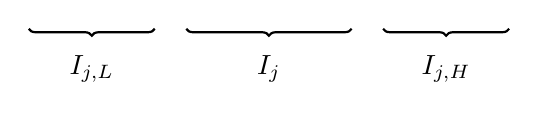
\begin{tikzpicture}[every text node part/.style={align=center}]
		
		\draw[black, thick, decoration = {brace,mirror,raise=0cm},decorate] (8,0) -- node[below=6pt] {$I_{j,L}$} (9.6,0);
		
		\draw[black, thick, decoration = {brace,mirror,raise=0cm}, decorate]
		(10,0) -- node[below=6pt] {$I_{j}$} (12.1,0);
		
		\draw[black, thick, decoration = {brace,mirror,raise=0cm},decorate] (12.5,0) -- node[below=6pt] {$I_{j,H}$} (14.1,0);
		
		\end{tikzpicture}
		
		\item Q is the operator that is defined as
		\begin{equation}
		Q \cdot R\cdot\hat{u} = \hat{u}\label{Q_operator_1}
		\end{equation}
		for any $\hat{u}$ that satisfies the border conditions. (Notice that $Q = R^{-1}$ if R is square, and this is only true as maps on functions which satisfy the boundary). Formally, we define $Q$ as a matrix of size $\hat{I} \times I$ given by:
		\begin{equation}
		Q = \begin{bmatrix}
		Q_1 & \mathbf{0}_1       & ...    & \mathbf{0}_1\\
		\mathbf{0}_2       & Q_2 & ...    & \mathbf{0}_2\\
		\vdots  & \vdots  & \ddots & \vdots \\
		\mathbf{0}_n       & \mathbf{0}_n       & ...    & Q_n\\
		\end{bmatrix}\label{Q_def}
		\end{equation}
		where, for any arbitrary $j$, $Q_j$ is a partitioned matrix of size $\hat{I_j} \times I_j$ given by:
		\begin{equation}
		Q_j = \begin{bmatrix}
		 &  & Q_{j,L} &   & \\
		 &  & \mathbb{I}_{(I_j \times I_j)} \\
		 &  & Q_{j,H} &   & \\
		\end{bmatrix}\label{Qj_def}
		\end{equation}
		whose submatrices $Q_{j,L}$ and $Q_{j,H}$ (of size $I_{j,L} \times I_j$ and $I_{j,H} \times I_j$, respectively) elements depend on the border conditions and the submatrix $\mathbb{I}_{(I_j\times I_j)}$ is an identity matrix of dimension $I_j$. 
		
		Q also has a second relation: 
		\begin{equation}
		B\cdot Q\cdot u  = \begin{bmatrix}
		\text{B}_{x^{1},L} & ... & \text{B}_{x^{N},L}\\
		\text{B}_{x^{2},H} & ... & \text{B}_{x^{N},H}
		\end{bmatrix}\hat{u}=\begin{bmatrix}
		\text{z}_{1, L}&\text{z}_{2, L}&\dots&\text{z}_{n, L}\\
		\text{z}_{1, H}&\text{z}_{2, H}&\dots&\text{z}_{n, H}
		\end{bmatrix}\label{Q_operator_2}
		\end{equation}
		basically saying that it's a map from discretizations of functions in the interior to functions which satisfy the border conditions. In order to hold on trivial $u$, we need that the interior of $Q$ is identity, so it is defined by its first and last rows.\\
		Q is actually in general affine, meaning that $Q\cdot \hat{u} = Q_a\cdot \hat{u} + Q_b$. For example, the definition given of inner product make $Q\cdot x=b$ in an iterative solver converge to $Q_a\cdot x = b - Q_b$. From the relations, $Q_a$ is $\hat{I}\times I$ and $Q_b$ is of length $\hat{I}$. In order for $Q\cdot R\cdot u = u$ to hold for trivial $\hat{u}$, we need that $Q_b$ is zero except in the boundary rows.
		
		\item Now let's focus on solving an expression like $\hat{u}^d = A \hat{u}$, where the superscript $d$ means the discretized version of the variable. Consider, with some abuse of notation, that such expression means both the discretized and non-discretized forms. Then we have two relations\footnote{We could not find a way to clearly show two relations above are correct, but some intuitions are provided in the text}:
		
		\begin{align}
		[A[:, 1:I_L] A[:,\hat{I}-I_H+1:\hat{I}]]\cdot\left([B[:,1:I_L] B[:,\hat{I}-I_H+1:\hat{I}]]^{-1}\begin{bmatrix}
		\text{b}_{x^{1},L} & ... & \text{b}_{x^{N},L}\\
		\text{b}_{x^{2},H} & ... & \text{b}_{x^{N},H}
		\end{bmatrix}\right) = A\cdot Q_b\label{affine_relation_1}
		\end{align}
		\begin{align}
		R(A-[A[:,1:I_L] A[:,\hat{I}-I_H+1:\hat{I}]]\cdot([B[:,1:I_L] B[:,\hat{I}-I_H+1:\hat{I}]]^{-1} B) = A\cdot Q_a\label{affine_relation_2}
		\end{align}
		
		Our intuition is that the main idea here is using interiors to recover a relation that boundary conditions should satisfy. Since $Q_b$ is a $\hat{I}\times 1$ matrix containing zeros excepts two ends, the two non-zero elements in $Q_b$ capture partial information of boundary nodes (the part that is ``independent'' of interiors).  Recall \eqref{B_operator_block}, so $\left([B[:,1:I_L] B[:,\hat{I}-I_H+1:\hat{I}]]^{-1}\begin{bmatrix}
		\text{b}_{x^{1},L} & ... & \text{b}_{x^{N},L}\\
		\text{b}_{x^{2},H} & ... & \text{b}_{x^{N},H}
		\end{bmatrix}\right)$ recovers the ``independent" part of boundary nodes. Then it is reasonable to expect that \eqref{affine_relation_1} holds.
		
		Multiply both sides of \eqref{affine_relation_2} by $\hat{u}$, we can roughly rewrite the relation as
		\begin{equation}
		R(A\cdot \hat{u}-A\cdot Q_b) = A\cdot Q_a\cdot \hat{u}
		\end{equation}
		so $A\cdot \hat{u}-A\cdot Q_b$ will be a discretized $\hat{u}$ which contains the entire information of interiors and the rest part of boundary information that is not covered by $A\cdot Q_b$. 
		
		However, we are not sure if $R$ should exist on the left of \eqref{affine_relation_2} since R by definition is a restriction operator and $R(A\cdot \hat{u}-A\cdot Q_b)$ only contains information from interiors. Also the size of the LHS of \eqref{affine_relation_2} is $I\times \hat{I}$, but the size of the RHS is $\hat{I}\times I$.
		For now, while we work on better understanding those expressions, we will take them as given.
		
		
		Given those relationships, in order to solve the differential equation, we now only have to solve for the interior. Otherwise, including the boundary values would imply having more points than there are degrees of freedom in the problem - thus making the numerical solution unstable. Moreover, the boundaries are given directly by the interior $\hat{u} = Qu$. 
		
		Therefore, we actually want to solve $\hat{u}^d = AQu$. Notice that the discretized A maps from the full domain to the interior\footnote{Notice that the PDE is only defined on the interior}. Notably, that means it's not square. Additionally, consider that, as described above, since $Q$ is in general affine, thus:
		\begin{equation}
		\hat{u} = AQ_au + AQ_b
		\end{equation}
	Those are the linear equations which define the ODE or whose solution is the solution to the PDE.
		
	This shows that what's important and non-trivial is $Q$. It contains all of the information about both the boundaries and the domain from the two relations. So what is Q? Here's all of the relevant cases for finite differencing:
	\begin{enumerate}
	\item \textbf{Dirichlet$_0$}: If you have any $v$ in the interior, its unique extension to satisfying the border conditions is sticking $0$'s on the ends, so both $Q_{j,L}$ and $Q_{j,H}$ are null matrices, i.e. block matrices in which all elements are zero. Therefore, Q is linear, meaning $Q = Q_a$ and $Q_b$ is a null matrix.
			
	\item \textbf{Dirichlet}: The boundary is not dependent on any points in the interior, and therefore $Q_a$ is identical to the previous case ($Q_{j,a} = [\textbf{0}_{(I_{j,L} \times I_j)}; \mathbb{I}_{(I_j \times I_j)} ; \textbf{0}_{(I_{j,H} \times I_j,)} ]$), but now Q is no longer linear and
	 $Q_{j,b}$ is given by 
	 $Q_{j,b} = [\text{B}_{j,L}[1,\dots,I_L,:]; \textbf{0}_{(I_j\times I_j)};
	\text{B}_{j,H}[\hat{I}_j - I_H,\dots,\hat{I},:]]$.
			
	\item \textbf{Neumann}: You have to pick a discretization of B. 
	This defines linear relation between the interior points and the boundary conditions. For example, for the univariate case, the first order discretization of the boundary derivative means that 
			
	\begin{equation}
		\frac{db}{dx} = \frac{\hat{u_j}[2] - \hat{u}[1]}{dx} = \text{B}[1,\dots,I_{L},:]
	\end{equation}
			
	and, therefore, $u[1] = u[2] - dx\text{B}[I_L,:]$. You can see that this implies that $Q_b = [dx\text{B}[I_L,:];\{0\}_1^I;dx \text{B}[I_H,:]]$ and that $Q_a$ is the identity matrix for the interior points and $[1,0, 0,...,0]$ for the first $I_L$ rows\footnote{So that $Q_a u = u[1] = \hat{u}[I_L+1]$.} and $[0,...,0,0,1]$ for the last $I_H$ rows.%\footnote{so that $Q_a v = v[1] = u[2]$ and $Q_a v = v[I] = u[I-1]$, respectively.}.
			
\end{enumerate}
\end{itemize}

\section{Time-Invariant Stochastic Process Examples}
Let $x_t$ be a stochastic process for a univariate function defined on a continuous domain $x \in (\underline{x}, \bar{x})$ where $-\infty < \underline{x} < \bar{x} < \infty$.  We will assume throughout that the domain is time-invariant.

For a given $\A$ Then, if the payoff in state $x$ is $b(x)$, and payoffs are discounted at rate $r > 0$, then the simple HJBE for $u(x)$ is,
\begin{align}
r u(x) &= b(x) + \A u(x)\label{eq:general-stationary-HJBE}
\end{align}
subject to $\D[x]u(\underline{x}) = 0$ and $\D[x]u(\bar{x}) = 0$ for reflecting barriers.  If it is a lower absorbing barrier, then denote $\D[x]u(\underline{x}) = \underline{u}$ which may be non-zero.

For a simple example of a payoff, choose $b(x) = x$.

\subsection{Stationary HJBE with Reflecting Barriers}
Take the stochastic process
$$
d x_t = d \W_t
$$
with reflecting barriers at $\underline{x}$ and $\bar{x})$.  The partial differential operator (infinitesimal generator) associated with the stochastic process is
$$
	\A \equiv \frac{1}{2}\D[xx]
$$

With this process,
\begin{itemize}
	\item How to derive all of the matrices of \cref{sec:general}
	\item The system of equations to solve for $u(x)$ in \cref{eq:general-stationary-HJBE}
	\item Check that the code \url{operator_examples\simple_stationary_HJBE_reflecting.jl} is correct
\end{itemize}
We can re-define the problem as 
\begin{align}
\mathcal{L} u(x) &= x\label{HJBE_reflecting_barriers_PDE}\\
\text{where }\mathcal{L}&\equiv r - \A
\end{align}
We first consider a one-dimension case where $x\in [0, 1]$. Let $I_L = I_H = 1$ and thereby $\Delta  = \frac{1}{\bar{I}}$ and $\hat{I} = I+2$. The matrix form of operator $\mathcal{L}$ can be defined as
\begin{equation}
L = r\cdot \mathbf{I}_{\hat{I}\times\hat{I}}-\underbrace{\begin{bmatrix}
-1&1&0&\dots&0&0&0\\
1&-2&1&\dots&0&0&0\\
\vdots&\vdots&\vdots&\ddots&0&0&0\\
0&0&0&\cdots&1&-2&1\\
0&0&0&\cdots&0&1&-1
\end{bmatrix}}_{\equiv A}\Delta^{-2}=
\begin{bmatrix}
r\Delta^2+1&-1&0&\dots&0&0&0\\
-1&r\Delta^2+2&-1&\dots&0&0&0\\
\vdots&\vdots&\vdots&\ddots&0&0&0\\
0&0&0&\cdots&-1&r\Delta^2+2&-1\\
0&0&0&\cdots&0&-1&r\Delta^2+1
\end{bmatrix}\Delta^{-2}
\end{equation}
where the dimension of A is $\hat{I}\times\hat{I}$.\\
Since $x\in[0, 1]$, we have boundary conditions 
\begin{align}
\mathcal{L} u(\underline{x}) &= 0\\
\mathcal{L} u(\bar{x})& = 1
\end{align}
Then we can define $B$ as
\begin{equation}
B\cdot\hat{u} =\underbrace{\begin{bmatrix}
r\Delta^2+1&-1&0&\dots&0&0&0\\
0&0&0&\cdots&0&-1&r\Delta^2+1
\end{bmatrix}}_{\equiv B}\cdot\hat{u} = \begin{bmatrix}
0\\
1
\end{bmatrix}
\end{equation}
where $\hat{u} = \begin{bmatrix}
u(x_0)\\
u(x_1)\\
\vdots\\
u(x_I)\\
u(x_{I+1})
\end{bmatrix}_{\hat{I}\times 1}$.\\
$R$ is defined as 
\begin{equation}
R\cdot \hat{u} =\begin{bmatrix}
0&1&0&\cdots&0&0\\
0&0&1&\cdots&0&0\\
\vdots&\vdots&\vdots&\ddots&\vdots&\vdots\\
0&0&0&\cdots&1&0
\end{bmatrix}_{I\times\hat{I}}\cdot \hat{u}		 
=\begin{bmatrix}
u(x_1)\\
u(x_2)\\
\vdots\\
u(x_I)
\end{bmatrix} \in \R^{I} 
\end{equation}
According to \eqref{HJBE_reflecting_barriers_PDE}, we can identify $x_0$ and $x_{I+1}$ by following relations
\begin{align}
&\begin{cases}
\begin{bmatrix}
-1&r\Delta^2+2&-1&\dots&0&0&0
\end{bmatrix}\cdot \hat{u} &= x_1\\
\begin{bmatrix}
0&0&0&\cdots&-1&r\Delta^2+2&-1
\end{bmatrix}\cdot \hat{u}& = x_I
\end{cases}\\
&\begin{cases}
u(x_0) &= (r\Delta^2+2)u(x_1)-u(x_2) - x_1\\
u(x_{I+1})&=(r\Delta^2+1)u(x_I)-u(x-{I_1})-x_I
\end{cases}
\end{align}
Thus, $Q$ is defined by $Q\cdot R\cdot\hat{u}\equiv Q_a\cdot R\cdot\hat{u}+Q_b = \hat{u}$, where
\begin{equation}
Q_a = \begin{bmatrix}
r\Delta^2+2&-1&\cdots&0&0\\
1&0&\cdots&0&0\\
0&1&\cdots&0&0\\
\vdots&\vdots&\ddots&\vdots&\vdots\\
0&0&\cdots&1&0\\
0&0&\cdots&0&1\\
0&0&\cdots&-1&r\Delta^2+2
\end{bmatrix}_{\hat{I}\times I}\quad\text{and}\quad Q_b = \begin{bmatrix}
-x_1\\
0\\
0\\
\vdots\\
0\\
0\\
-x_{I}
\end{bmatrix}_{\hat{I}\times 1}
\end{equation}
Then we should be able to express $\hat{u}$ in terms of $A$, $B$, $R$, and $Q$ as in \eqref{affine_relation_1} and \eqref{affine_relation_2}.

\subsection{Stationary HJBE with a Lower Absorbing Barrier}
Take the stochastic process
$$
d x_t = d \W_t
$$
with an absorbing barrier at $\underline{x}$, and a reflecting barrier at $\bar{x})$.  The partial differential operator (infinitesimal generator) associated with the stochastic process is
$$
\A \equiv \frac{1}{2}\D[xx]
$$

For the absorbing barrier, when solving for the HJBE assume that $u(\underbar{x}) = \underbar{x}$ and $u'(\bar{x}) = 0$


With this process,
\begin{itemize}
	\item How to derive all of the matrices of \cref{sec:general}
	\item The system of equations to solve for $u(x)$ in \cref{eq:general-stationary-HJBE}
	\item Check that the code \url{operator_examples\simple_stationary_HJBE_reflecting.jl} is correct
\end{itemize}


\subsection{Stationary HJBE with Only Drift}
Now, do the same after adding in constant drift (and manually choose the correct upwind direction!)
$$
d x_t = \mu dt
$$
With a generator
$$
	\A \equiv \mu \D[x]
$$
With this process,
\begin{itemize}
	\item How to derive all of the matrices of \cref{sec:general}.  Be careful to use the appropriate upwind direction for the first order term.
	\item The system of equations to solve for $u(x)$ in \cref{eq:general-stationary-HJBE}
	\item Write julia code to solve for $u(x)$ with the grid
	\item Check these for $\mu < 0$ and $\mu > 0$.
\end{itemize}


\subsection{Stationary HJBE with Reflecting Barriers and Drift}
Now, do the same after adding in constant drift (and manually choose the correct upwind direction!)
$$
d x_t = \mu dt + \sigma d\W_t
$$
With a generator
$$
	\A \equiv \mu \D[x] + \frac{\sigma^2}{2}\D[xx]
$$
With this process,
\begin{itemize}
	\item How to derive all of the matrices of \cref{sec:general}.  Be careful to use the appropriate upwind direction for the first order term.
	\item The system of equations to solve for $u(x)$ in \cref{eq:general-stationary-HJBE}
	\item Write julia code to solve for $u(x)$ with the grid
	\item Check these for $\mu < 0$ and $\mu > 0$.
\end{itemize}



\subsection{Stationary Bellman Equation with Reflecting Barriers State Varying Drift/Variance}
Now, do the same after adding in constant drift (and manually choose the correct upwind direction!)
$$
d x_t = \mu(x_t) dt + \sigma(x_t) d\W_t
$$
With a generator
$$
\A \equiv \mu(x) \D[x] + \frac{\sigma(x)^2}{2}\D[xx]
$$
With this process,
\begin{itemize}
	\item How to derive all of the matrices of \cref{sec:general}.  Be careful to use the appropriate upwind direction for the first order term.
	\item The system of equations to solve for $u(x)$ in \cref{eq:general-stationary-HJBE}
	\item Write julia code to solve for $u(x)$ with the grid.
	\begin{itemize}
		\item Choose a $\mu(x)$ and $\sigma(x)$ functions, consider using geometric brownian motion as a test.  That is,
		\begin{align}
			\A &\equiv \bar{\mu} x \D[x] + \frac{\bar{\sigma}^2}{2}x^2\D[xx]
		\end{align}
	\end{itemize}
\end{itemize}

\end{document}
